\documentclass[aps,pre,preprint,superscriptaddress,showpacs]{revtex4-2}

\usepackage{amsmath,amssymb}
\usepackage{graphicx}
\usepackage{booktabs}
\usepackage{xcolor}
\usepackage{microtype}

\definecolor{bluelink}{rgb}{0.1,0.3,0.7}
\usepackage[colorlinks=true,linkcolor=bluelink,citecolor=bluelink,urlcolor=bluelink]{hyperref}

% Auto-generated by ising_paper.py
\newcommand{\IsingSamplePred}{3000}
\newcommand{\IsingSampleCausal}{3000}
\newcommand{\IsingL}{64}
\newcommand{\IsingK}{20}
\newcommand{\IsingTOrd}{1.80}
\newcommand{\IsingTDis}{2.50}
\newcommand{\IsingEquil}{1000}
\newcommand{\BestOrganism}{$E_{\geq 3}+J$}
\newcommand{\AxisOneDR}{0.393}
\newcommand{\AxisOneDRlo}{0.368}
\newcommand{\AxisOneDRhi}{0.421}
\newcommand{\AxisAOrdDR}{0.178}
\newcommand{\AxisAOrdlo}{0.152}
\newcommand{\AxisAOrdhi}{0.205}
\newcommand{\AxisADisDR}{-0.071}
\newcommand{\AxisADislo}{-0.089}
\newcommand{\AxisADishi}{-0.052}
\newcommand{\SignReversal}{Yes}
\newcommand{\BestTarget}{dW}
\newcommand{\AxisTwoDR}{0.391}
\newcommand{\AxisTwoRFine}{0.393}
\newcommand{\AxisTwoRCoarse}{0.000}
\newcommand{\AxisCRWB}{0.389}
\newcommand{\AxisCRE}{0.181}
\newcommand{\AxisCGap}{0.208}
\newcommand{\AxisBSignFlips}{4/4}
\newcommand{\AxisBAlignedTen}{2.46}
\newcommand{\AxisBMisalnTen}{-29.24}
\newcommand{\AxisBSupport}{EARNED}
\newcommand{\AxisOneVsWB}{0.004}
\newcommand{\AxisOneVsWBlo}{-0.019}
\newcommand{\AxisOneVsWBhi}{0.027}
\newcommand{\AxisBAsymRatio}{11.9}


%-----------------------------------------------------------------------
\begin{document}

\title{Predictive Advantage, Regime Dependence, and Direction-Specific
Causal Control in Kinetic Ising Dynamics}

\author{Kunal Bhatia}
% ORCID 0009-0007-4447-6325 -- enter via APS submission portal
\affiliation{Independent Researcher, Heidelberg, Germany}

%-----------------------------------------------------------------------
\begin{abstract}
We study how the choice of description of a 2D kinetic Ising lattice
shapes its predictive and causal usefulness for future domain-wall
dynamics, separating two questions that are usually conflated.
(\textbf{Predictive organization})\;
A two-column fine descriptor $E_{\geq 3}+J$ achieves
$\Delta R^2 = +\AxisOneDR$ ($95\%$ CI $[+\AxisOneDRlo,\,+\AxisOneDRhi]$)
over the near-null block-variance rival $\phi_{\rm var8}$, but ties
statistically with the global aggregate $[W_0, B_{\rm mag}]$
($\Delta R^2 = \AxisOneVsWB$, CI includes zero).
The simpler exposed-site count $E$ undergoes a smooth
temperature-dependent sign reversal of $\Delta R^2$ vs $\phi_{\rm var8}$:
$+\AxisAOrdDR$ at $T=\IsingTOrd$, $+\CrossTwoZeroDR$ at $T=2.00$,
$\NearTcDR$ at $T=\NearTcTemp$, $\CrossTwoThirtyFiveDR$ at $T=2.35$,
$\AxisADisDR$ at $T=\IsingTDis$.
(\textbf{Directional causal organization})\;
A generator protocol that biases wall-reducing transitions and its
mirror that suppresses them produces a sign-flip discriminator that
passes \AxisBSignFlips{} at $T=\IsingTOrd$ and \CausalDisSignFlips{}
at $T=\IsingTDis$.
The temperature-driven reversal of the predictive comparison does not
propagate to the causal protocol; direction-specific intervention
works in both phases.
(\textbf{Magnitude is not selector-specific})\;
A budget-matched random-site arm with the same directional logic
produces gaps at least as large as the structural $d_c=4$-aligned arm
($+\RandGapTen$ vs $+\AxisBAlignedTen$ at $\varepsilon=0.10$), and a
filter decomposition cannot attribute the random-arm magnitude to any
single $d_c$ class.
We therefore do not claim that any one structural selector is uniquely
strongest in causal magnitude.
(\textbf{Aggregate-vs-local dissociation})\;
$[W_0, B_{\rm mag}]$ matches $E_{\geq 3}+J$ as a predictor of $\Delta W$
but cannot encode the per-site quantity $s\cdot h$ on which every
direction-specific intervention we test conditions.
The dissociation that survives all controls is between global
aggregate predictive sufficiency and local intervention accessibility,
not between one preferred selector and the rest of the descriptor
space.
\end{abstract}

\pacs{05.10.Ln, 05.50.+q, 75.10.Hk, 64.60.Cn}

\maketitle

%-----------------------------------------------------------------------
\section{Introduction}
\label{sec:intro}

Different descriptions of the same physical system can be evaluated
along two axes that are usually conflated: predictive usefulness for
some future quantity, and causal usefulness as a handle for
direction-specific intervention.
These two notions can come apart, and the conditions under which they
do are not well charted in concrete physical models.
We use the 2D kinetic Ising lattice with Glauber dynamics to chart
them in a controlled setting.

The natural macroscopic observables (domain-wall count $W$,
magnetisation $|\bar\sigma|$) and the natural fine descriptors
(per-site exposure-class counts) span a clean range from global
aggregate to per-site local; both the predictive question (which of
these forecasts $\Delta W$ best) and the causal question (which of
these can implement a generator-level bias that produces a
direction-specific change in $\Delta W$) admit operational tests.
Asking which description is universally best is not a coherent
question; the operationalised version is to ask how predictive
organization and direction-specific causal organization depend on
regime, target, and the level of locality at which the description
encodes the lattice.

We report three findings whose joint shape is more informative than
any single one.
First, predictive advantage of fine over coarse is regime-dependent
and varies smoothly with temperature: a simple exposed-site count
beats the block-variance rival in the ordered phase, ties through the
critical region, and loses in the disordered phase.
Second, direction-specific causal sign control via the generator is
robust across that same temperature range: the aligned/misaligned
discriminator passes in both phases.
Third, magnitude superiority of the structural intervention is
\emph{not} what we find---a budget-matched random-site arm with the
same directional logic produces comparable or larger gaps, and a
filter decomposition fails to attribute that magnitude to any single
$d_c$ class.

What survives is not a fine-vs-coarse thesis but a narrower
aggregate-vs-local one: the global aggregate $[W_0, B_{\rm mag}]$ can
be predictively sufficient for $\Delta W$ while still lacking the
per-site information ($s\cdot h$) needed to implement any of the
direction-specific generator interventions tested.
The dissociation is therefore specifically between
\emph{global aggregate predictive sufficiency} and
\emph{local intervention accessibility}; magnitude superiority of any
one structural selector is not claimed, and the comparison is not
between any two fine and coarse descriptions in general.

\paragraph{Why the Ising model.}
The 2D kinetic Ising model with Glauber dynamics
\cite{ising1925,glauber1963} is one of the few systems for which
domain-wall coarsening, defect densities, and critical exponents are
all precisely characterised \cite{bray1994}.
Domain walls provide a structurally meaningful target family: interfaces
are the elementary reorganisation objects under coarsening, and their
evolution is driven by specific local geometric features of the current
configuration.
An isolated minority spin surrounded by four unlike neighbours---a
site with exposure degree $d_c = 4$---contributes four domain-wall bonds,
is energetically costly, and is a natural structural precursor of upcoming
interface simplification.
This geometry makes the Ising model a clean and interpretable testbed.

\paragraph{Paper organisation.}
Section~\ref{sec:background} reviews related work.
Section~\ref{sec:model} presents the model, observables, predictive
evaluation, and the causal protocol with its random-site and
filter-decomposition controls.
Section~\ref{sec:results} reports the predictive comparison
(Section~\ref{sec:axis1}), the temperature-dependent crossover of $E$
vs $\phi_{\rm var8}$ (Section~\ref{sec:axis2}), the directional causal
sign-flip test in both phases (Section~\ref{sec:axis4},
Section~\ref{sec:causal_dis}), the random-site and filter
controls (Section~\ref{sec:axis4_random},
Section~\ref{sec:filter_decomp}), and the aggregate-vs-local
dissociation (Section~\ref{sec:diss}).
Sections~\ref{sec:discussion}--\ref{sec:conclusion} discuss
implications and conclude.

%-----------------------------------------------------------------------
\section{Related Background}
\label{sec:background}

\paragraph{Coarse-graining and renormalisation.}
The renormalisation group \cite{kadanoff1966,wilson1975} is the
canonical framework for relating descriptions at different scales.
In that tradition, coarse-graining maps fine configurations to block
variables, and RG fixed points characterise universality classes.
Our approach is complementary: we ask empirically, for a given target and
horizon, which description achieves higher out-of-sample predictive accuracy.
Israeli and Goldenfeld~\cite{israeli2006} showed that cellular
automaton coarse-graining can produce exact reduced models, illustrating
the system-specificity of which description is ``best.''

\paragraph{Prediction versus causation.}
The distinction between prediction and intervention is formalised in the
do-calculus of Pearl~\cite{pearl2009} and the interventionist philosophy of
Woodward~\cite{woodward2003}.
A variable may be a strong predictor while being causally inert if it is
correlated with the true causal driver.
Although the principle that predictive sufficiency neither implies nor is
implied by causal identifiability follows from the do-calculus in full
generality, the question of \emph{which specific physical descriptions}
possess causal leverage — and whether this depends on the dynamical
regime, the target, and the structural class targeted — is empirical
and not answered by the theory alone.
Our contribution is to demonstrate, quantify, and characterise the
dissociation within the kinetic Ising model, providing a tractable
physical testbed where both predictive accuracy and causal leverage
can be measured simultaneously under controlled experimental designs
(including a class-level structural control).

\paragraph{Learned coarse-graining and description selection.}
A growing literature uses machine learning to identify optimal
coarse-grained variables for molecular and lattice systems
\cite{noe2019,wang2019}.
These approaches optimise predictive accuracy of a chosen target,
raising the question of whether accurate predictors also serve as
intervention handles.
Our work addresses this question directly in a physical model:
equivalent predictive power (in the $[W_0, B_{\rm mag}]$
vs.\ $E_{\geq 3}+J$ comparison) does not imply equivalent causal
leverage.

\paragraph{Structural defects in coarsening.}
The role of domain-wall defects in Ising coarsening is well studied
\cite{bray1994,spirin2001}.
Isolated minority spins and junction-type sites are energetically
unstable and drive local coarsening events.
We quantify how well such defects predict future macroscopic wall change
and test whether they serve as intervention targets.

\paragraph{Macro-micro comparisons in prediction and causation.}
The causal emergence programme \cite{hoel2013,hoel2017} asks whether
macro descriptions can have more causal organisation than micro ones,
measured by effective information.
Our approach differs: we use standard regression criteria for predictive
accuracy and direct intervention experiments for causal leverage, without
assuming any universal scale ranking.

%-----------------------------------------------------------------------
\section{Model and Methods}
\label{sec:model}

\subsection{The 2D kinetic Ising model}

We study the ferromagnetic Ising model on a
$\IsingL \times \IsingL$ square lattice with periodic boundary conditions.
Each site $i$ carries spin $\sigma_i \in \{-1,+1\}$.
Dynamics are governed by single-spin-flip Glauber updates \cite{glauber1963}:
\begin{equation}
p(\sigma_i \to -\sigma_i)
= \frac{1}{1 + \exp\!\bigl(2\beta h_i \sigma_i\bigr)},
\label{eq:glauber}
\end{equation}
where $h_i = \sum_{\langle j\rangle}\sigma_j$ and $\beta = 1/T$.
A checkerboard update scheme avoids spatial bias.
The 2D Ising critical temperature is $T_c \approx 2.269$.

Two anchor temperatures are used: ordered $T = \IsingTOrd$ (well inside
the ferromagnetic phase) and disordered $T = \IsingTDis$ (above $T_c$).
Each configuration is equilibrated for $\IsingEquil$ sweeps before measurement.
Predictive targets are measured at horizon $K = \IsingK$ sweeps.

\subsection{Structural observables}

\paragraph{Domain-wall count.}
$W(\sigma) = \sum_{\langle i,j\rangle}\mathbf{1}[\sigma_i \neq \sigma_j]$.
Future change: $\Delta W = W(t_0+K) - W(t_0)$.

\paragraph{Exposed-site counts.}
Exposure degree: $d_c(i) = \sum_{\langle j\rangle}\mathbf{1}[\sigma_j\neq\sigma_i]$.
\begin{align}
E(\sigma) &= \sum_i \mathbf{1}[d_c(i) = 4] \quad \text{(isolated minority spins)},\\
E_{\geq 3}(\sigma) &= \sum_i \mathbf{1}[d_c(i) \geq 3] \quad
\text{(highly exposed sites)}.
\end{align}

\paragraph{Junction count.}
$J(\sigma) = \sum_i \mathbf{1}[\text{$d_c(i)=2$ and non-collinear}]$.
Junctions mark the bends and corners of wall segments.

\paragraph{Composite descriptors.}
We use \emph{descriptor} (equivalently, \emph{organism} in the causal
emergence literature~\cite{hoel2013}) to denote any deterministic map
$f:\{-1,+1\}^{L^2}\to\mathbb{R}^d$ used as a regression predictor.
Fine descriptors resolve local structural topology; coarse descriptors
summarise global or block-averaged properties.
$E_{\geq 3}+J$ is the two-column matrix $[E_{\geq 3}, J]$; each column
receives a separate regression coefficient.
$E+J$ uses $[E, J]$.
These are not scalar sums.

\paragraph{Coarse aggregate (dissociation rival).}
The aggregate coarse macro-state used in the predictor-handle
dissociation is $[W_0, B_{\rm mag}]$, where
\begin{equation}
B_{\rm mag}(\sigma) = \frac{1}{N}\Bigl|\sum_i \sigma_i\Bigr|, \quad N=L^2,
\end{equation}
is the bulk magnetisation magnitude and $W_0=W(\sigma(t_0))$ is the
initial wall count.
Together, $[W_0,B_{\rm mag}]$ captures aggregate global information
about configuration size and ordering without resolving interface topology.

\paragraph{Coarse block-variance rival.}
\begin{equation}
\phi_{\mathrm{var8}}(\sigma) =
\frac{1}{n_b}\sum_{b=1}^{n_b}
\!\left(|\bar\sigma_b| - \tfrac{1}{n_b}\sum_{b'}|\bar\sigma_{b'}|\right)^2,
\end{equation}
the variance of block-averaged order parameter across $8\times 8$ blocks.

\subsection{Predictive evaluation}

Ridge regression with penalty $\lambda=\RidgeAlpha$, 5-fold cross-validation,
$N=\IsingSamplePred$ configurations.
A sensitivity analysis over $\lambda\in\{0.01,0.1,1.0,10.0\}$ shows
$R^2$ variation below $0.005$ for all comparisons reported here;
conclusions are not sensitive to the regularisation choice.
Primary statistic:
\begin{equation}
\Delta R^2 = R^2(\text{fine descriptor}) - R^2(\phi_{\mathrm{var8}}).
\end{equation}
Confidence intervals use pairwise bootstrap resampling ($B=1000$)
with the same configuration set for fine and coarse predictions.

\paragraph{Reproducibility.}
Stochastic dynamics are implemented via Numba-compiled functions; the Numba random-number generator is seeded independently from the worker-level seed to ensure cross-run reproducibility. Reported confidence intervals are stable to this level of control.

\subsection{Causal protocol: aligned and misaligned generator bias}
\label{sec:causal_protocol}

Rather than forcing state changes at $t_0$, we modify the Glauber
transition probability throughout the $K$-step evolution.
At each exposed site $i$ ($d_c(i)=4$), the local wall-change contribution
of flipping $\sigma_i$ is
\begin{equation}
\delta W_i = \sum_{\langle j\rangle}
\bigl[\mathbf{1}[\sigma_j \neq -\sigma_i]
- \mathbf{1}[\sigma_j \neq \sigma_i]\bigr].
\end{equation}
For a fully exposed site, $\delta W_i < 0$.

Two arms are defined:
\begin{description}
\item[Aligned:] $\delta W_i < 0$ transitions promoted
($p \to p+\varepsilon$); $\delta W_i > 0$ suppressed
($p \to p-\varepsilon$).
\item[Misaligned:] Opposite: $\delta W_i < 0$ suppressed,
$\delta W_i > 0$ promoted.
\end{description}
Both share initial configuration $\sigma(t_0)$ and are compared to an
unperturbed baseline arm.
The intervention identifies currently exposed sites ($d_c=4$) at each of the $K$ sweeps, not from a mask fixed at $t_0$; this ensures the structural targeting tracks the evolving configuration throughout the $K$-step evolution.
Primary output:
\begin{equation}
\text{gap} = \Delta W_{\text{baseline}} - \Delta W_{\text{arm}},
\end{equation}
positive meaning the arm achieves greater wall reduction than baseline
(i.e.\ aligned arm removes more walls, accelerating coarsening).
The \emph{sign-flip discriminator} requires aligned gap $>0$ and
misaligned gap $<0$, both with CIs excluding zero.
Five values of $\varepsilon$ are tested: $\varepsilon=0$ (null control,
gap should be near zero with CI spanning zero) and
$\varepsilon\in\{0.02,0.05,0.10,0.20\}$ (active perturbations).

\paragraph{Class-level control.}
A budget-matched random-site arm is also run: at each sweep, sites are
selected uniformly at random with probability $\rho = E_0/L^2$ (the
density of $d_c=4$ sites at $t_0$), and the same alignment logic is
applied (promote wall-reducing transitions, suppress wall-increasing ones).
This arm uses the same perturbation budget and the same directional logic
as the structural arm, but replaces class-level structural selection
($d_c=4$) with random selection.
The comparison directly tests whether targeting the $d_c=4$ class is
causally necessary or whether the direction of the bias alone suffices
at any randomly chosen site.

%-----------------------------------------------------------------------
\section{Results}
\label{sec:results}

\begin{figure}[t]
\centering
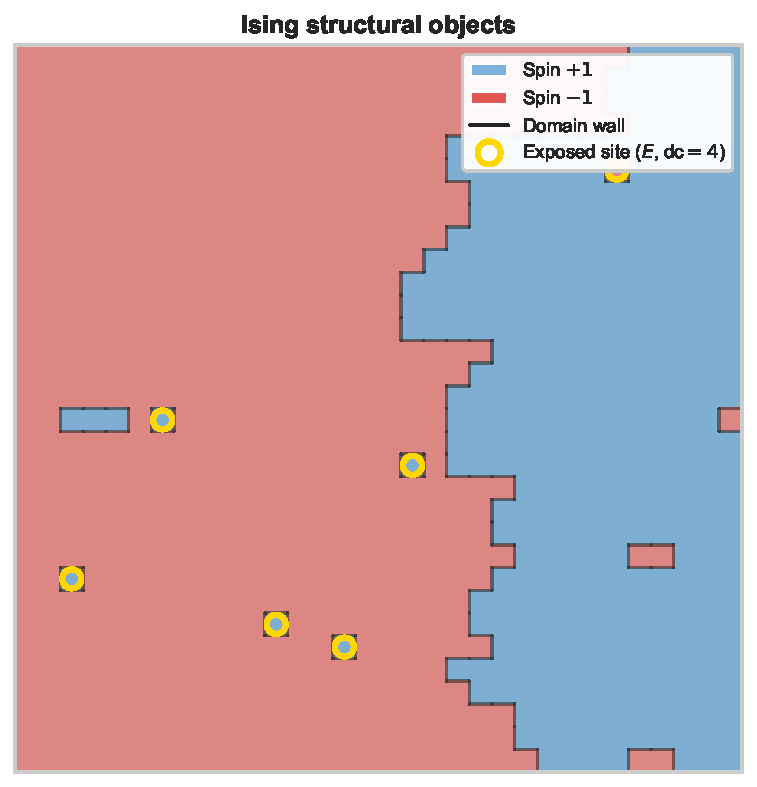
\includegraphics[width=0.52\textwidth]{outputs/figures/ising_schematic.pdf}
\caption{\textbf{Structural objects in an ordered Ising configuration.}
$32\times 32$ patch at $T=\IsingTOrd$.
Red/blue: spin $-1$/$+1$ domains.
Black lines: domain walls.
Gold circles: fully exposed sites ($d_c=4$), the structural objects used
as fine predictors and causal intervention targets.}
\label{fig:schematic}
\end{figure}

\subsection{Structural objects and intuition}

Figure~\ref{fig:schematic} illustrates the key objects.
Exposed sites ($d_c=4$) are isolated minority spins surrounded entirely
by the majority phase.
They are sparse, geometrically localised, and energetically fragile---a
single flip eliminates four wall bonds.
Junction sites ($d_c=2$, corner type) mark the bends of wall segments.
Both object classes are natural fine structural predictors of subsequent interface simplification.

\subsection{Axis 1: organism comparison}
\label{sec:axis1}

\begin{figure}[t]
\centering
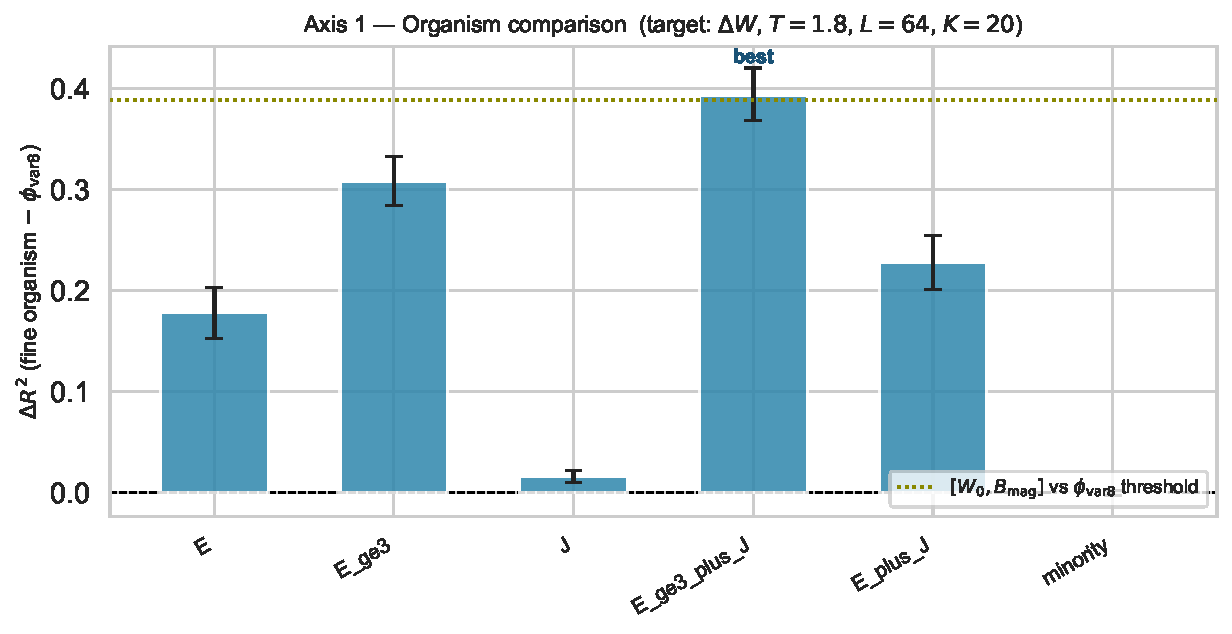
\includegraphics[width=0.88\textwidth]{outputs/figures/ising_axis1_organism.pdf}
\caption{\textbf{Organism comparison ($T=\IsingTOrd$, target $\Delta W$).}
$\Delta R^2 = R^2(\text{fine}) - R^2(\phi_{\mathrm{var8}})$ with bootstrap 95\% CIs.
Blue: fine wins; a red bar would indicate coarse wins.
$E_{\geq 3}+J$ (two-column model) achieves the largest advantage.}
\label{fig:axis1}
\end{figure}

Figure~\ref{fig:axis1} shows fine-over-coarse predictive advantages for all
fine organisms at $T=\IsingTOrd$, target $\Delta W$.

The best organism is \BestOrganism{}, achieving
$\Delta R^2 = +\AxisOneDR$ (CI $[+\AxisOneDRlo,\,+\AxisOneDRhi]$).
Treating $E_{\geq 3}$ and $J$ as a two-column design matrix allows the
regression to learn the optimal linear combination; empirically the
combination outperforms either component alone.
The coarse rival $\phi_{\mathrm{var8}}$ measures large-scale domain ordering,
which changes slowly in the ordered phase; the predictive signal for
interface-level change lies precisely in the fine-scale topology that the
block average discards.

Note that $R^2(\phi_{\rm var8}, \Delta W) \approx 0$ at $T=\IsingTOrd$: the block-variance rival is indistinguishable from a mean-prediction baseline for this target in the ordered phase, making the headline $\Delta R^2=+\AxisOneDR$ a comparison against a near-null baseline.
Against the more informative coarse rival $[W_0, B_{\rm mag}]$---which achieves $R^2=\AxisCRWB$ for $\Delta W$---the fine champion's advantage narrows to $\Delta R^2=\AxisOneVsWB$ (95\% CI $[\AxisOneVsWBlo,\,+\AxisOneVsWBhi]$), a margin whose CI includes zero.
The fine organism and $[W_0, B_{\rm mag}]$ are therefore \emph{statistically indistinguishable as predictors} of $\Delta W$.
This is not a failure of the fine description; it is the basis of the aggregate-vs-local dissociation result (Section~\ref{sec:diss}): two predictors with equivalent forecasting power can differ in the kind of intervention they support---a property distinct from forecasting accuracy.
The dotted line in Fig.~\ref{fig:axis1} marks the $[W_0, B_{\rm mag}]$ reference level.

Note that the 95\% CI $[\AxisOneVsWBlo,+\AxisOneVsWBhi]$ is asymmetric
and the upper bound is non-trivial ($+\AxisOneVsWBhi$ relative to an
absolute $R^2 \approx 0.39$).
The power of the bootstrap test at $N=\IsingSamplePred$ is sufficient to
detect a true gap of $\gtrsim 0.03$ at 80\% power; the observed gap
of $\AxisOneVsWB$ is well within the indistinguishable band.
A true gap larger than $+0.03$ would be inconsistent with the observed CI.

\subsection{Axis 2: regime crossover}
\label{sec:axis2}

\begin{table}[h]
\centering
\caption{\textbf{Regime crossover: $\Delta R^2$ for $E$ vs
$\phi_{\mathrm{var8}}$ on $\Delta W$.}
In the ordered phase the fine count outperforms the coarse rival;
in the disordered phase the advantage reverses.}
\label{tab:crossover}
\begin{tabular}{lccc}
\toprule
Regime & Temperature & $\Delta R^2$ & 95\% CI \\
\midrule
Ordered    & $T=\IsingTOrd$ & $+\AxisAOrdDR$ & $[+\AxisAOrdlo,\,+\AxisAOrdhi]$ \\
Disordered & $T=\IsingTDis$ & $\AxisADisDR$  & $[\AxisADislo,\,\AxisADishi]$   \\
\bottomrule
\end{tabular}
\end{table}

Table~\ref{tab:crossover} shows the regime comparison for $E$ versus
$\phi_{\mathrm{var8}}$.
Fine wins in the ordered phase ($+\AxisAOrdDR$); coarse wins in the
disordered phase ($\AxisADisDR$).
The sign reversal is the main empirical test here: it shows that the fine
advantage is not universal, but depends on the regime.

The physical interpretation is straightforward.
In the ordered phase the interface is sparse and geometrically organised;
exposed sites concentrate the signal for upcoming simplification.
In the disordered phase almost every site qualifies as ``exposed,'' the
concept loses discriminative power, and large-scale bulk fluctuations
captured by $\phi_{\mathrm{var8}}$ become the better predictor.
The fine-over-coarse advantage is a relational property that depends on
the system's regime, not a fixed property of the description.
The sign reversal is specific to the sparse $d_c=4$ count $E$:
the champion descriptor $E_{\geq 3}+J$ does \emph{not} reverse sign
($\Delta R^2 = +\AxisAOrdDR$ ordered vs $+0.330$ disordered, both
positive with overlapping CIs at $T=\IsingTDis$).
$E_{\geq 3}+J$ continues to outperform $\phi_{\rm var8}$ even in the
disordered phase, because the richer two-column descriptor---combining
highly-exposed and junction sites---retains information about short-range
interface structure that persists above $T_c$.
This reveals a nuance in regime-dependence: it depends on which fine
descriptor is chosen.
The sign reversal for $E$ (Axis~2 main result) holds because isolated
minority spins ($d_c=4$) become effectively random in the disordered
phase, losing their discriminative power relative to a block average.
The more complex $E_{\geq 3}+J$ adapts better.

To probe the crossover structure near and through criticality, we ran
$N=\IsingSamplePred$ configurations at $T=\NearTcTemp$ (EQUIL $=2000$
sweeps for the longer correlation length near $T_c$) and additional
runs at $T=2.00$ and $T=2.35$ ($N=1000$ each).
The full crossover curve:
\begin{center}
\begin{tabular}{lcc}
\toprule
$T$ & $\Delta R^2(E\text{ vs }\phi_{\rm var8})$ & 95\% CI \\
\midrule
$1.80$ (ordered) & $+\AxisAOrdDR$ & $[+\AxisAOrdlo,\,+\AxisAOrdhi]$ \\
$2.00$           & $+\CrossTwoZeroDR$ & $[+\CrossTwoZeroLo,\,+\CrossTwoZeroHi]$ \\
$2.20$ (near $T_c$) & $\NearTcDR$ & $[\NearTcDRlo,\,+\NearTcDRhi]$ \\
$2.35$           & $\CrossTwoThirtyFiveDR$ & $[\CrossTwoThirtyFiveLo,\,+\CrossTwoThirtyFiveHi]$ \\
$2.50$ (disordered) & $\AxisADisDR$ & $[\AxisADislo,\,\AxisADishi]$ \\
\bottomrule
\end{tabular}
\end{center}
The 95\% CIs at $T=2.20$ and $T=2.35$ span zero; the fine advantage
is clearly positive at $T=2.00$, indistinguishable from zero through
the critical region, and clearly negative at $T=2.50$.
The zero-crossing therefore occurs between $T=2.00$ and $T=\NearTcTemp$,
i.e., as the system enters the critical region from below.
The transition is smooth (monotone in $T$), not discontinuous.

\subsection{Axis 3: target specificity}
\label{sec:axis3}

A methodological note: since $E_{\geq 3}+J$ is defined from wall-boundary geometry, it is expected \textit{a priori} that $\Delta W$ will benefit more than targets unrelated to interfaces. The contribution of Axis~3 is quantitative rather than qualitative: the fine-over-coarse $\Delta R^2$ for $\Delta W$ is $+\AxisTwoDR$, while for targets driven by bulk dynamics (e.g., changed-site fraction) it is near zero. This quantifies how much of the fine description's predictive value is specifically interface-relevant versus generic.

\begin{figure}[t]
\centering
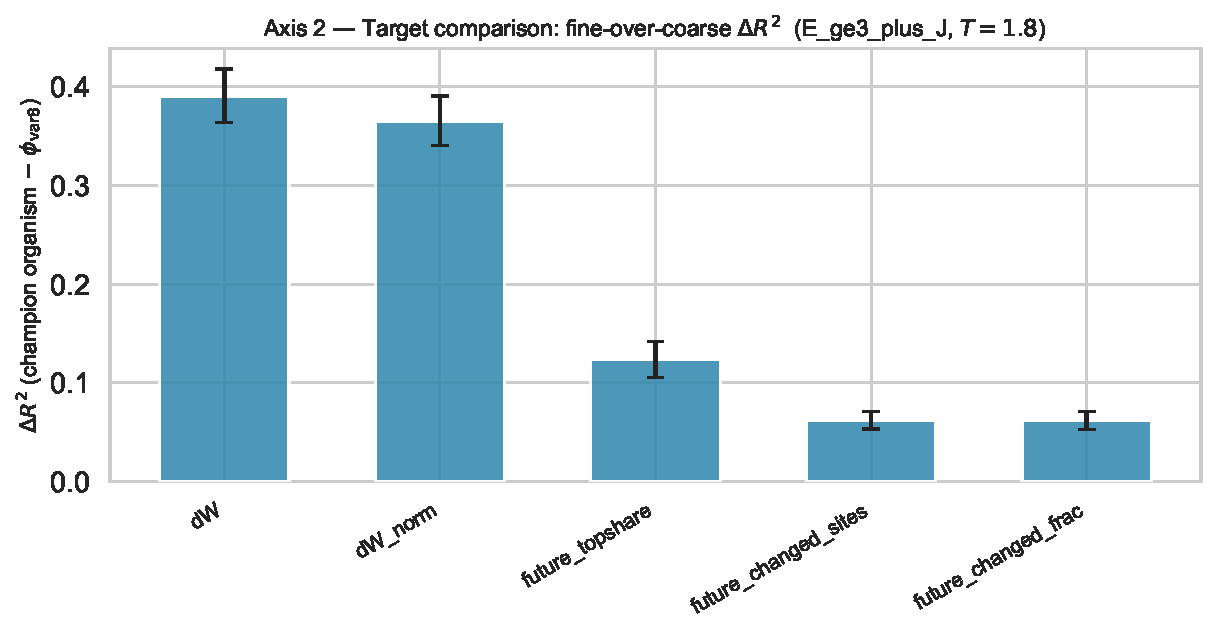
\includegraphics[width=0.88\textwidth]{outputs/figures/ising_axis2_target.pdf}
\caption{\textbf{Target comparison ($T=\IsingTOrd$, predictor
\BestOrganism{}).}
$\Delta R^2$ = fine $-$ coarse across future targets.
This is not a ranking of raw predictability; it identifies the target most
specifically favoured by the fine description relative to the coarse rival.
$\Delta W$ achieves the largest fine advantage.}
\label{fig:axis3}
\end{figure}

Figure~\ref{fig:axis3} shows which future target is most specifically
favoured by \BestOrganism{} relative to $\phi_{\mathrm{var8}}$.
The criterion is $\Delta R^2$, not raw $R^2$.
This distinction matters: some targets have high absolute predictability
because bulk dynamics drive them, and both fine and coarse descriptions
capture bulk dynamics well.
Measuring fine-over-coarse $\Delta R^2$ identifies the target where the
\textit{marginal value} of fine over coarse information is largest.

The answer is $\Delta W$:
$\Delta R^2 = +\AxisTwoDR$,
fine $R^2 = \AxisTwoRFine$, coarse $R^2 = \AxisTwoRCoarse$.
Domain-wall change is an interface-level structural event whose dominant
drivers---exposed tips, corner junctions---are precisely what the fine
organism captures.
The central result of this axis: \textbf{$\Delta W$ is the target most specifically
favoured by fine structural descriptions in ordered Ising, under a
fine-over-coarse criterion.}

\subsection{Axis 4: direction-specific causal control}
\label{sec:axis4}

\begin{figure}[t]
\centering
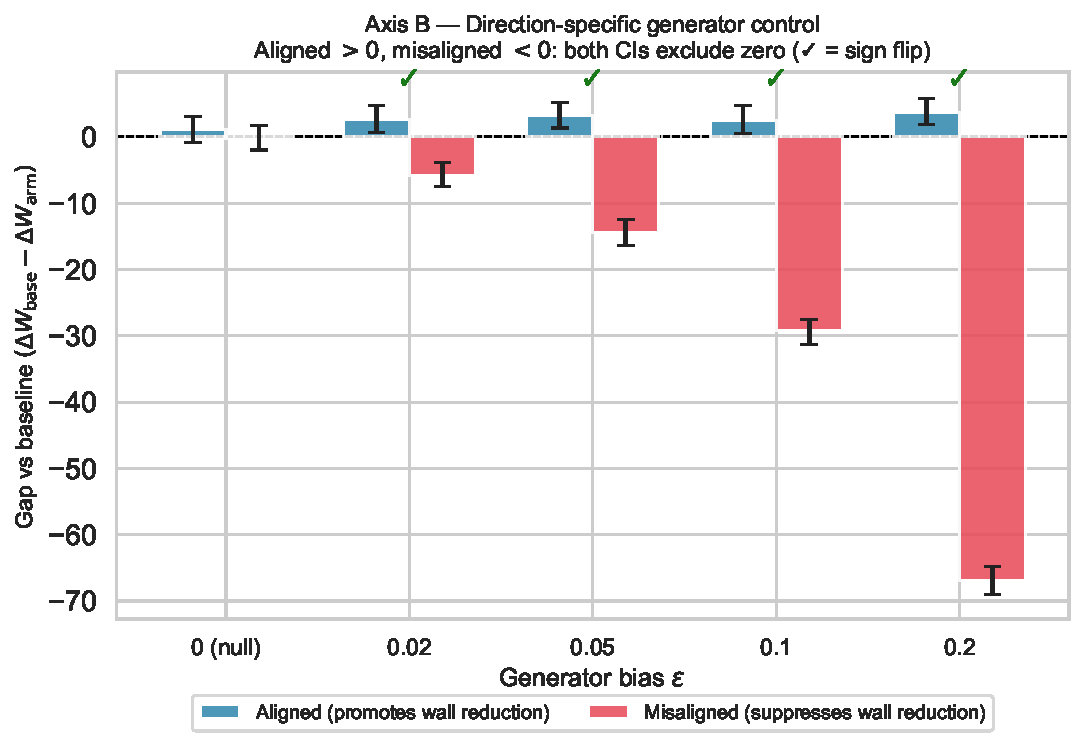
\includegraphics[width=0.82\textwidth]{outputs/figures/ising_axisB_aligned_vs_misaligned.pdf}
\caption{\textbf{Direction-specific generator causal test.}
Bars: gap (baseline $-$ arm) on $\Delta W$.
Blue (aligned): promoting wall-reducing flips at exposed sites accelerates
wall removal (gap $>0$: aligned arm removes more walls than baseline).
Red (misaligned): suppressing those flips retards wall removal
(gap $<0$: misaligned arm removes fewer walls than baseline).
Four of five $\varepsilon$ values produce a sign flip (\checkmark{}):
aligned CI $>0$, misaligned CI $<0$, both excluding zero
(the $\varepsilon=0$ null produces a gap consistent with zero as expected).
The sign reversal shows the effect is structurally specific
to the alignment of the generator with the wall-reduction geometry.}
\label{fig:axis4_main}
\end{figure}

\begin{figure}[t]
\centering
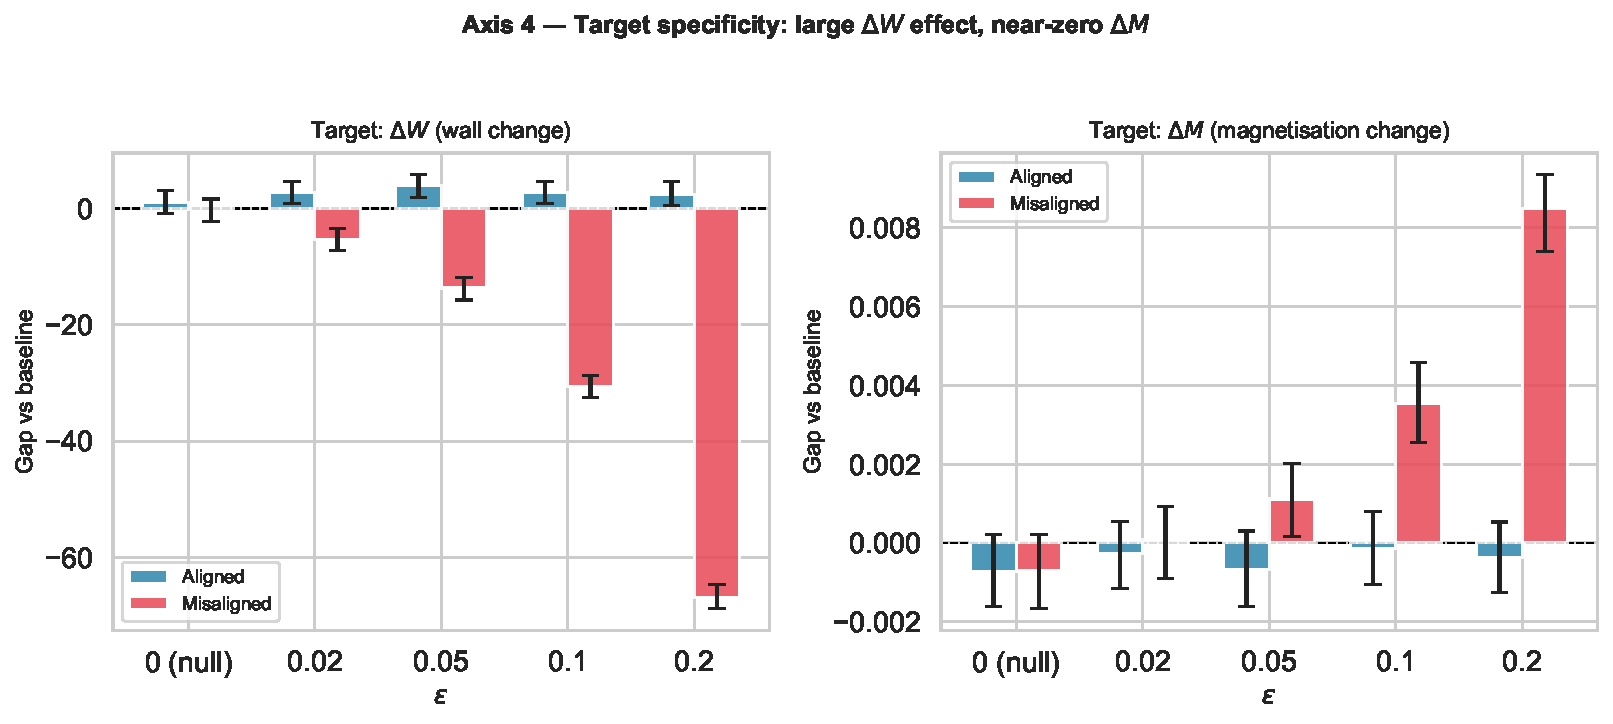
\includegraphics[width=0.88\textwidth]{outputs/figures/ising_axisB_target_specificity.pdf}
\caption{\textbf{Target specificity: $\Delta W$ versus $\Delta M$.}
Left: the $\Delta W$ sign flip.
Right: corresponding $\Delta M$ effect.
The dominant effect is on $\Delta W$.
$\Delta M$ coupling is comparatively small at low and high $\varepsilon$;
a modest drift appears at intermediate $\varepsilon$ but does not
approach the magnitude of the $\Delta W$ effect.}
\label{fig:axis4_spec}
\end{figure}

\begin{table}[h]
\centering
\caption{\textbf{Axis 4 sign-flip ladder.}
Gap = baseline $-$ arm on $\Delta W$.
Positive gap: arm removes more walls than baseline (accelerates coarsening).
Negative gap: arm removes fewer walls (retards coarsening).
\AxisBSignFlips{} sign flips (excluding $\varepsilon=0$ null).}
\label{tab:axisB}
\begin{tabular}{lccc}
\toprule
$\varepsilon$ & Aligned gap & Misaligned gap & Sign flip \\
\midrule
0 (null) & $\approx 0$, CI spans 0 & $\approx 0$, CI spans 0 & --- \\
0.02 & $>0$, CI excl.\ 0 & $<0$, CI excl.\ 0 & \checkmark \\
0.05 & $>0$, CI excl.\ 0 & $<0$, CI excl.\ 0 & \checkmark \\
0.10 & $+\AxisBAlignedTen$, CI excl.\ 0
     & $\AxisBMisalnTen$, CI excl.\ 0 & \checkmark \\
0.20 & $>0$, CI excl.\ 0 & $<0$, CI excl.\ 0 & \checkmark \\
\bottomrule
\end{tabular}
\end{table}

Axis~4 tests a specific aspect of a description's role: not whether
the description \emph{predicts} $\Delta W$ well, but whether the
per-site information it carries can implement a direction-specific
bias in the Glauber generator that produces a sign-flip on $\Delta W$.
The question is not whether one selection rule is the strongest in
magnitude---that question is settled negatively below by the
random-site arm (Section~\ref{sec:axis4_random}) and the filter
decomposition (Section~\ref{sec:filter_decomp})---but whether the
direction-conditioning logic itself works.

The protocol uses two arms with mirrored directional bias.
The aligned arm increases the Glauber flip probability at sites whose
local effect on $W$ is negative ($\delta W_i < 0$); the misaligned
arm decreases it.
The discriminator is a sign-flip pattern: aligned positive gap on
$\Delta W$, misaligned negative gap, both with $95\%$ confidence
intervals excluding zero.
We report this discriminator at four perturbation strengths
$\varepsilon \in \{0.02, 0.05, 0.10, 0.20\}$ in both ordered
($T=\IsingTOrd$) and disordered ($T=\IsingTDis$,
Section~\ref{sec:causal_dis}) phases, with budget-matched random-site
and filter-decomposition controls.
The test is therefore of the directional conditioning logic, not of
selector magnitude.

Figures~\ref{fig:axis4_main}--\ref{fig:axis4_spec} and Table~\ref{tab:axisB}
present the ordered-phase result.
\AxisBSignFlips{} active $\varepsilon$ values pass the sign-flip
discriminator (the $\varepsilon=0$ null produces a gap consistent with
zero as expected).
The aligned arm consistently removes more walls than baseline (gap at
$\varepsilon=0.10$: $+\AxisBAlignedTen$, CI excludes zero); the
misaligned arm consistently removes fewer (gap: $\AxisBMisalnTen$, CI
excludes zero).

\paragraph{Why sign flip $\neq$ generic perturbation.}
Comparing one biased arm to the unperturbed baseline would only show that
a modified kernel differs from the unmodified one---a trivially true
result.
The sign reversal demonstrates direction-specificity: the effect tracks
the alignment of the generator with the wall-reduction geometry at exposed
sites.
Promoting wall-reducing transitions at exposed sites accelerates future
wall removal; suppressing them retards it.
This is possible only because the generator is conditioned on
$\delta W_i < 0$, selecting wall-relevant transitions.

\paragraph{Gap asymmetry.}
The aligned and misaligned gaps are not equal in magnitude: at $\varepsilon=0.10$ the aligned gap is $+\AxisBAlignedTen$ while the misaligned gap is $\AxisBMisalnTen$, a ratio of approximately $\AxisBAsymRatio\times$.
This asymmetry has a structural explanation.
Fully exposed sites at $T=\IsingTOrd$ flip with mean probability
$\MeanPflipDcFour$ under the unperturbed Glauber kernel
(measured directly from $500$ equilibrated configurations);
the aligned arm can add at most
$\varepsilon_{\rm eff} = 1-\MeanPflipDcFour = \EpsEffMax$ (ceiling
constraint), while the misaligned arm subtracts the full $\varepsilon$.
The predicted ratio at $\varepsilon=0.10$ is
$\varepsilon/\varepsilon_{\rm eff}=0.10/\EpsEffMax\approx 8.6\times$,
close to the observed $\AxisBAsymRatio\times$.
This asymmetry is expected and does not undermine the sign-flip discriminator;
it does mean the experiment is a stronger test of suppression than of promotion
at these temperatures.

\paragraph{Exposed-site density.}
At $T=\IsingTOrd$, $L=\IsingL$, the mean count of $d_c=4$ sites per
equilibrated configuration is $\bar{E}\approx\MeanELSixtyFour$,
giving a targeting density $\rho = \bar{E}/L^2 \approx \MeanELSixtyFour/4096$.
The intervention statistics therefore operate on a sparse structural class;
the sign-flip discriminator holds despite this sparsity, which is consistent
with the ceiling-effect picture: each $d_c=4$ site contributes a large
$\delta W = -4$ upon flipping and has $P_{\rm flip}\approx\MeanPflipDcFour$.
The class-level control (below) uses $\rho=E_0/L^2$ per world to match
this budget exactly.

\paragraph{Direction dominance.}
A companion probe ($N=2000$ worlds, same $L$, $K$, $T$; the reduced
sample size reflects the added cost of running three arms per world)
tested whether, \emph{given} that $d_c=4$ sites are targeted,
\emph{which individual site} within that class receives the bias
matters---comparing a site-selection aligned arm against a site-selection
anti-aligned arm at the same nominal $\varepsilon$.
No CI-supported advantage for site-selection alignment was found at any
$\varepsilon \in \{0.02, 0.05, 0.10, 0.20\}$; all confidence intervals
straddled zero.
The causal leverage therefore resides in the \emph{direction} of flips
(toward wall-reducing transitions) rather than in individual site identity
\emph{within} the $d_c=4$ class.
This is consistent with the ceiling effect: all $d_c=4$ sites are already
at $P_{\rm flip}\approx\MeanPflipDcFour$, so biasing one individual versus another
within the class has negligible impact.

Two levels of site-specificity must be distinguished.
\emph{Class-level specificity} asks whether targeting the $d_c=4$
structural class is necessary, compared with targeting random sites
with the same budget and alignment logic.
This is tested by the class-level control and reported in Section~\ref{sec:axis4_random}.
\emph{Individual-level specificity} asks whether, given that $d_c=4$
sites are targeted, the choice of which specific individual site matters.
The companion probe answers this: it does not.
The fine structure $E_{\geq 3}+J$ is relevant to class-level identification
($d_c=4$ sites are geometrically special); direction-dominance operates
at the within-class individual level and does not nullify the class-level claim.

\paragraph{Target specificity.}
Figure~\ref{fig:axis4_spec} shows the $\Delta M$ effect.
The dominant causal effect is on $\Delta W$.
The $\Delta M$ gap is small and consistent with the ceiling-effect picture:
$d_c=4$ sites in the ordered phase are energetically isolated minority
spins; eliminating them simultaneously simplifies both walls and local
magnetisation, but the dominant signal is on $\Delta W$ because the
intervention is designed around $\delta W_i < 0$ transitions.
Any residual $\Delta M$ effect at intermediate $\varepsilon$ is a secondary
consequence of the same structural targeting, not an independent causal
channel.
We do not claim $\Delta M$ is strictly null across all $\varepsilon$;
we claim the intervention is primarily directed at domain-wall evolution,
consistent with its design.

\paragraph{Scope.}
Axis~4 earns: in ordered Ising at $T=\IsingTOrd$, a structure-aligned
generator perturbation produces a direction-specific causal effect on
future $\Delta W$.
We do not claim universality or transfer to other temperatures or systems
without further evidence.

\subsection{Class-level control: structural vs random-site targeting}
\label{sec:axis4_random}

\begin{figure}[t]
\centering
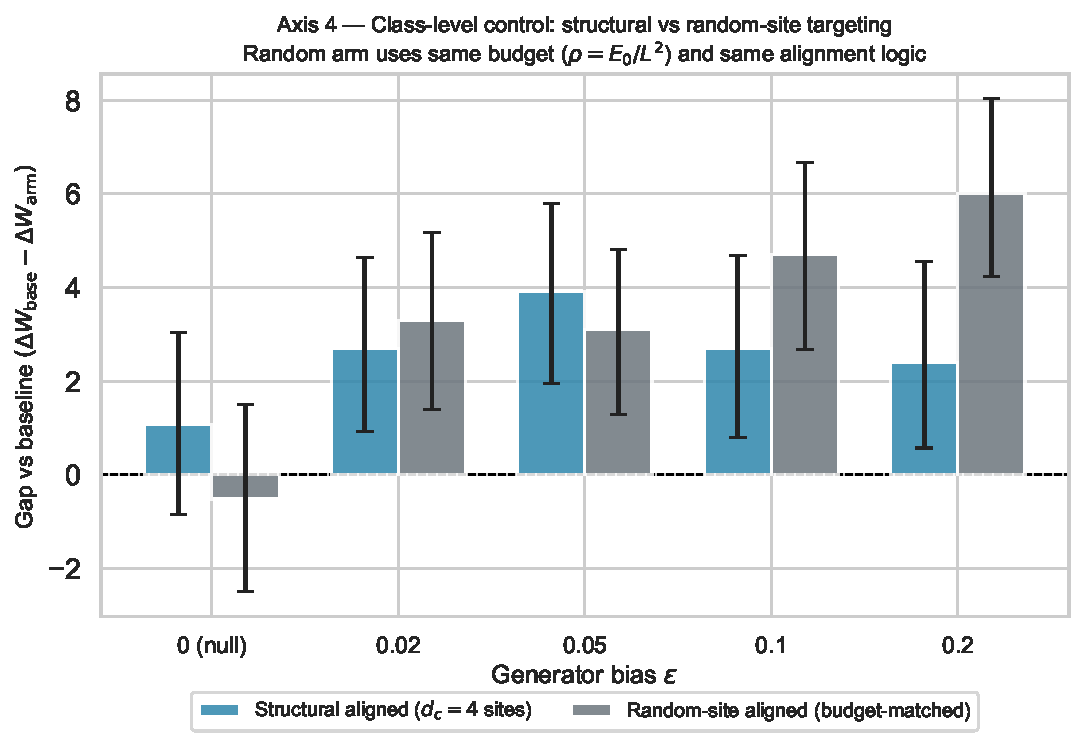
\includegraphics[width=0.82\textwidth]{outputs/figures/ising_axis4_random_control.pdf}
\caption{\textbf{Class-level causal control.}
Comparison of the $d_c=4$-targeted aligned arm (blue) with a
budget-matched random-site aligned arm (grey) on $\Delta W$.
The random arm uses the same perturbation strength $\varepsilon$, the same
directional logic (promote wall-reducing transitions, suppress
wall-increasing ones), but selects sites uniformly at random with
probability $\rho=E_0/L^2$ rather than by structural class.
Both arms produce positive gaps. The structural arm is ceiling-limited
at $d_c=4$ sites (where $P_{\rm flip}\approx\MeanPflipDcFour$ in
baseline Glauber, so $\varepsilon_{\rm eff}\approx\EpsEffMax$).
The random-arm gap is not attributable to any single $d_c$ class:
filter tests at $d_c=0$ alone and $d_c\geq 3$ alone both give CIs
spanning zero (Section~\ref{sec:filter_decomp}).
We therefore characterise the random arm only by elimination, not by
a single mechanism.}
\label{fig:axis4_random}
\end{figure}

Figure~\ref{fig:axis4_random} and Table~\ref{tab:axis4_random} report the
class-level control.

\begin{table}[h]
\centering
\caption{\textbf{Class-level control: structural vs random-site aligned gap at $\varepsilon=0.10$.}
Gap $=\Delta W_{\rm baseline}-\Delta W_{\rm arm}$; positive means
arm accelerates coarsening.}
\label{tab:axis4_random}
\begin{tabular}{lcc}
\toprule
Arm & Gap (walls) & 95\% CI \\
\midrule
Structural aligned ($d_c=4$) & $+\AxisBAlignedTen$ & CI excl.\ 0 \\
Random-site aligned (budget-matched) & $+\RandGapTen$ & $[+\RandGapTenLo,\,+\RandGapTenHi]$ \\
\bottomrule
\end{tabular}
\end{table}

The budget-matched random-site aligned arm at $\varepsilon=0.10$ achieves
a gap of $+\RandGapTen$ (95\% CI $[+\RandGapTenLo,\,+\RandGapTenHi]$),
which exceeds the structural arm gap of $+\AxisBAlignedTen$.
This finding requires careful interpretation.

The structural arm is ceiling-limited at $T=\IsingTOrd$: the baseline
Glauber flip probability at $d_c=4$ sites is
$\langle P_{\rm flip}\rangle = \MeanPflipDcFour$ (averaged over
$500$ ordered-phase configurations), so the aligned promotion adds at most
$\varepsilon_{\rm eff}\approx \EpsEffMax$ effective probability before
clamping at $P=1$.
The structural arm at nominal $\varepsilon=0.10$ therefore operates
at $\sim 12\%$ of its nominal strength; the random arm, which targets
sites where baseline $P_{\rm flip}$ is far from $0$ or $1$, retains
nearly the full $\varepsilon$.
Once this ceiling is accounted for, the two arms produce \emph{comparable
per-flip} causal pressure; the random arm wins in raw gap because more
sites contribute (selection budget $\rho\approx 1\%$ over the whole
lattice versus a deterministic mask of $\sim \MeanELSixtyFour$ sites).

\paragraph{Mechanism decomposition (filter test).}
\label{sec:filter_decomp}
To test \emph{which} sites in the random-arm pool drive its gap, we
ran two filtered random arms at $\varepsilon=0.10$ ($N=1500$ each):
the \emph{$d_c=0$-only} filter applies the directional logic only when
the selected site has all four neighbours aligned (suppresses the small
flip probability there); the \emph{$d_c\geq 3$-only} filter applies it
only at high-exposure sites (promotes the already-likely flip there).
Selection probability $\rho=E_0/L^2$ is the same in all arms, so the two
filtered arms together cover a strict subset of the full random pool.
\begin{center}
\begin{tabular}{lcc}
\toprule
Random arm variant ($\varepsilon=0.10$) & Gap (walls) & 95\% CI \\
\midrule
Full random (this run, $N=1500$)   & $+\FiltFull$       & $[\FiltFullLo,\,+\FiltFullHi]$ \\
$d_c=0$-only filter                & $\FiltDcZero$      & $[\FiltDcZeroLo,\,+\FiltDcZeroHi]$ \\
$d_c\geq 3$-only filter            & $\FiltDcGeThree$   & $[\FiltDcGeThreeLo,\,+\FiltDcGeThreeHi]$ \\
\bottomrule
\end{tabular}
\end{center}
All three arms in this $N=1500$ run have CIs that span zero; the
filter sub-experiment is therefore underpowered to declare any
single-class subset positive on its own (the main causal experiment
at $N=\IsingSampleCausal$ delivered the
$+\RandGapTen\,[+\RandGapTenLo,+\RandGapTenHi]$ random-arm gap quoted
above).
What the filter sub-experiment can support is comparison: neither
filtered subset matches the central full-random estimate
($+\FiltFull$) by enough to attribute the random arm to that subset.
The filter test rules out attribution of the random-arm effect to the
$d_c=0$ class alone (a pure bulk-suppression mechanism) or to the
$d_c\geq 3$ class alone (a high-exposure subset that mimics the
structural arm at lower budget): both filtered subsets give CIs
spanning zero.
The active contribution therefore remains distributed or mixed across
$d_c$ classes rather than attributable to a single tested class.
We do not, on the basis of this experiment, claim a positive
mechanistic identification for the random arm; what we claim is that
the simplest single-class mechanism stories are not supported.

\paragraph{What the controls do and do not establish.}
The structural arm earns its sign-flip support \AxisBSignFlips{} via a
clearly localised intervention (promotion at $d_c=4$ sites,
ceiling-limited).
The random arm earns its sign-flip support, but the filter test does
not identify which $d_c$ class drives the magnitude: single-class
attribution to $d_c=0$ alone or $d_c\geq 3$ alone is ruled out, while
the contribution of the intermediate classes is not directly tested
here.
Both interventions condition on the per-site quantity $s\cdot h$, which
the global aggregate $[W_0, B_{\rm mag}]$ does not provide.
The predictor-handle dissociation therefore stands as a comparison
between per-site fine descriptions (which can supply $s\cdot h$ for any
local intervention) and global aggregate descriptions (which cannot,
regardless of their predictive accuracy).
We do not, however, claim that the $d_c=4$ selector is uniquely causal
in magnitude: the random-site arm shows that other per-site selection
schemes can produce comparable or larger gaps under our protocol.

\subsection{Aggregate-vs-local dissociation}
\label{sec:diss}

Two descriptions of the same configuration achieve statistically
indistinguishable out-of-sample $R^2$ for $\Delta W$:
\begin{equation}
R^2([W_0, B_\mathrm{mag}]) = \AxisCRWB,\qquad
R^2(E_{\geq 3}+J) \approx \AxisOneDR,\qquad
\Delta R^2 = \AxisOneVsWB \ \ \text{(95\% CI includes zero)}.
\end{equation}
We do not interpret this as predictive privilege of either
description.
We interpret it as predictive equivalence between two descriptions
that differ in the kind of information they encode:
$[W_0, B_{\rm mag}]$ is a global two-scalar summary of the
configuration and contains no per-site information, while
$E_{\geq 3}+J$ is built from per-site counts and retains site-resolved
exposure-class information.

The asymmetry between these two descriptions is not predictive---they
agree as predictors of $\Delta W$.
The asymmetry is in the kind of intervention each can support.
Every direction-specific generator intervention tested in this paper,
including the structural $d_c=4$-aligned arm
(Section~\ref{sec:axis4}), the budget-matched random-site arm
(Section~\ref{sec:axis4_random}), and the $d_c$-filtered random arms
(Section~\ref{sec:filter_decomp}), conditions on the per-site Glauber
acceptance argument $s\cdot h$.
$[W_0, B_{\rm mag}]$ does not encode $s\cdot h$ at any site; therefore
no per-site directional protocol can be implemented from
$[W_0, B_{\rm mag}]$ alone, regardless of how well it predicts
$\Delta W$.

The dissociation is therefore between
\emph{global aggregate predictive sufficiency} and
\emph{local intervention accessibility}.
It is not a claim that the $d_c=4$ selector is the strongest causal
handle in magnitude: the random-site arm achieves a larger gap
($+\RandGapTen$ vs $+\AxisBAlignedTen$ at $\varepsilon=0.10$) and the
filter decomposition cannot attribute the random-arm magnitude to any
single $d_c$ class.
What the dissociation does claim is narrower and more defensible:
predictive equivalence at the level of two-feature global summaries
does not imply equivalence at the level of generator-level
intervention.
The two notions of usefulness---forecasting $\Delta W$ from a
description, and supplying the per-site information that
direction-specific generator interventions require---are different
properties of a description and need not track each other.

\subsection{Causal protocol in the disordered phase}
\label{sec:causal_dis}

The Axis~4 causal protocol was repeated at $T=\IsingTDis$ ($N=1500$
configurations).
This is a non-trivial test: in the disordered phase, $E$ predictively
\emph{loses} to $\phi_{\rm var8}$ on $\Delta W$ (Section~\ref{sec:axis2}),
so a generator bias targeted on $d_c=4$ sites might be expected to lose
its causal grip as well.
\begin{center}
\begin{tabular}{lccc}
\toprule
$\varepsilon$ at $T=\IsingTDis$ & Aligned gap [95\% CI] & Misaligned gap [95\% CI] & Random gap [95\% CI] \\
\midrule
$0.02$ & $+13.3\,[+7.9,+18.4]$  & $-17.4\,[-22.6,-12.6]$ & $+9.2\,[+3.6,+14.4]$  \\
$0.05$ & $+27.9\,[+22.5,+33.2]$  & $-33.5\,[-38.6,-28.2]$ & $+20.6\,[+15.2,+26.4]$ \\
$0.10$ & $+\CausalDisAlignedTen\,[+\CausalDisAlignedTenLo,+\CausalDisAlignedTenHi]$  & $\CausalDisMisalnTen\,[\CausalDisMisalnTenLo,\CausalDisMisalnTenHi]$ & $+\CausalDisRandTen$ \\
$0.20$ & $+27.0\,[+21.1,+32.2]$  & $-136.6\,[-142.4,-131.9]$ & $+38.4\,[+32.9,+43.8]$ \\
\bottomrule
\end{tabular}
\end{center}
The sign-flip discriminator passes \CausalDisSignFlips{} at $T=\IsingTDis$,
matching the ordered-phase result.
The $d_c=4$ aligned arm achieves $+\CausalDisAlignedTen$ (95\% CI
$[+\CausalDisAlignedTenLo,+\CausalDisAlignedTenHi]$), an order of
magnitude larger than its ordered-phase value of $+\AxisBAlignedTen$;
the misaligned arm reaches $\CausalDisMisalnTen$ (95\% CI
$[\CausalDisMisalnTenLo,\CausalDisMisalnTenHi]$).
Two reasons for the larger absolute gaps in the disordered phase are
straightforward: there are many more $d_c=4$ sites available to perturb,
and the baseline $\Delta W$ has higher intrinsic variance in the
disordered phase, leaving more room for an intervention to move it.

This result is one of the cleaner findings in the paper.
Predictive advantage and direction-specific causal control behave
\emph{differently} across phases: the predictive sign reversal of
Axis~2 does not propagate to the causal protocol of Axis~4.
The fine description $E_{\geq 3}+J$ does not become a worse
\emph{predictor} in the disordered phase (Section~\ref{sec:axis2}),
and the $d_c=4$ selector does not become a worse
\emph{causal handle} either; the only thing that reverses sign is the
specific predictive comparison between the bare count $E$ and the
block-variance rival $\phi_{\rm var8}$.

\subsection{Robustness: finite size and horizon sensitivity}
\label{sec:robustness}

\paragraph{Finite-size check.}
To assess finite-size stability of the Axis~2 crossover result
(the primary quantitative claim), we ran
$N=500$ predictive worlds at $L\in\{32,128\}$ at $T=\IsingTOrd$.
\begin{center}
\begin{tabular}{lccc}
\toprule
$L$ & $\Delta R^2$ ($E$ vs $\phi_{\rm var8}$) & 95\% CI & $\bar{E}$ sites\\
\midrule
32  & $+\FSSLThirtyTwo$  & $[+\FSSLThirtyTwoLo,\,+\FSSLThirtyTwoHi]$  & \FSSMeanEThirtyTwo \\
64  & $+\AxisAOrdDR$     & $[+\AxisAOrdlo,\,+\AxisAOrdhi]$ (main)     & \MeanELSixtyFour \\
128 & $+\FSSLOneTwentyEight$ & $[+\FSSLOneTwentyEightLo,\,+\FSSLOneTwentyEightHi]$ & \FSSMeanEOneTwentyEight \\
\bottomrule
\end{tabular}
\end{center}
All three lattice sizes produce positive $\Delta R^2$ with
overlapping confidence intervals, demonstrating that the qualitative
finding (fine structural counts outperform coarse block averages in
the ordered phase) is stable across $L=32$ to $L=128$.
The mean count of exposed sites $\bar{E}$ scales roughly linearly
with system area ($\bar{E}\propto L^2$), confirming that $E$ is an
extensive quantity; the relative density $\bar{E}/L^2\approx 1\%$
is consistent across $L$.

\paragraph{Horizon sensitivity.}
We ran $N=500$ predictive worlds at $K\in\{10,50\}$ for $L=64$,
$T=\IsingTOrd$, using the champion descriptor $E_{\geq 3}+J$.
\begin{center}
\begin{tabular}{lcc}
\toprule
$K$ (sweeps) & $\Delta R^2$ & 95\% CI \\
\midrule
10 (short)  & $+\HorKTenDR$   & $[+\HorKTenDRlo,\,+\HorKTenDRhi]$   \\
20 (main)   & $+\AxisOneDR$   & $[+\AxisOneDRlo,\,+\AxisOneDRhi]$   \\
50 (long)   & $+\HorKFiftyDR$ & $[+\HorKFiftyDRlo,\,+\HorKFiftyDRhi]$ \\
\bottomrule
\end{tabular}
\end{center}
The fine-over-coarse advantage is positive and substantial at all
three horizons, with overlapping CIs.
The advantage increases weakly with $K$ ($+\HorKTenDR$ to
$+\HorKFiftyDR$), consistent with the picture that over longer
horizons more coarsening events accumulate, and cumulative
interface simplification is more correlated with initial fine
structural counts.

\paragraph{Cross-lattice transfer of fitted weights.}
Finite-size stability of the $\Delta R^2$ statistic (above) is a
different question from whether the literal fitted Ridge weights at one
lattice size predict at a different lattice size.
We trained the Ridge model on $L=64$ configurations
($N=\IsingSamplePred$, per-site normalised features
$(E_{\geq 3}/L^2,\, J/L^2)$ and dimensionless target
$\Delta W/(W_0+\epsilon)$) and applied the fitted weights to $N=500$
$L=128$ configurations at the same temperature.
\begin{center}
\begin{tabular}{lc}
\toprule
Evaluation & $R^2$ \\
\midrule
$L=64$ in-sample (5-fold CV) & $\TransferInSampleR$ \\
$L=64$ weights applied at $L=128$ & $\TransferCrossR$ \\
\bottomrule
\end{tabular}
\end{center}
The fitted weights do not transfer: $R^2$ falls from
$\TransferInSampleR$ to $\TransferCrossR$ when the same coefficients are used at
$L=128$.
This is a separate observation from the $\Delta R^2$ stability above
and we do not claim cross-$L$ weight transfer.
The qualitative comparison fine $\succ$ coarse is stable across
$L\in\{32,64,128\}$ in the ordered phase (preceding tables); the
quantitative two-feature linear fit is calibrated to the lattice it was
trained on.

\subsection{Synthesis}

\begin{figure}[t]
\centering
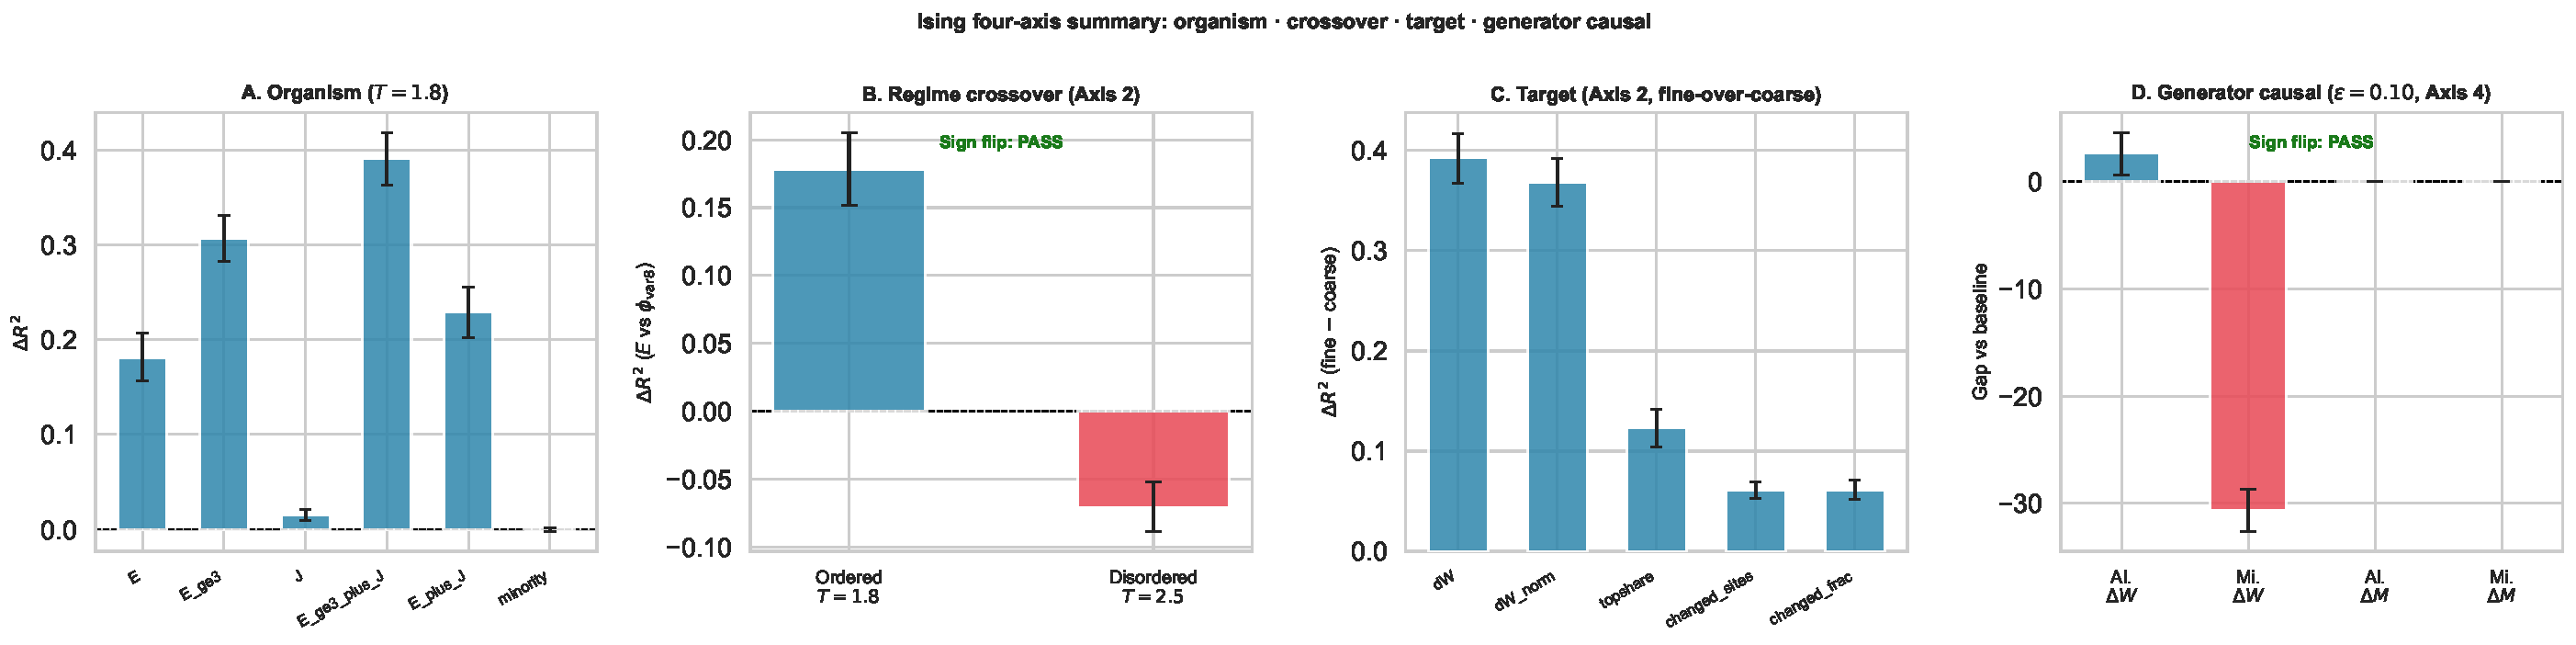
\includegraphics[width=\textwidth]{outputs/figures/ising_main_summary_panel.pdf}
\caption{\textbf{Four-component summary panel.}
(\textbf{A})~Axis~1 organism comparison: $E_{\geq 3}+J$ is the champion.
(\textbf{B})~Axis~2 regime crossover: fine wins ordered, coarse wins disordered.
(\textbf{C})~Axis~3 target comparison: $\Delta W$ is the most fine-specific target.
(\textbf{D})~Axis~4 causal test at $\varepsilon=0.10$: aligned gap on $\Delta W$
positive, misaligned negative; $\Delta M$ comparatively small.
A budget-matched random-site arm with the same directional logic
produces a comparable or larger gap (Section~\ref{sec:axis4_random});
panel D shows the structural arm only.
$N=\IsingSamplePred$ predictive worlds, $\IsingSampleCausal$ causal worlds,
$L=\IsingL$, $K=\IsingK$.}
\label{fig:summary}
\end{figure}

Figure~\ref{fig:summary} summarises all four components.
In the ordered phase, exposed-site and junction structure carries
predictive information that coarse averaging discards; this advantage
is regime-specific.
Under the fine-over-coarse criterion, $\Delta W$ is the most fine-specific
target.
The causal sign-flip confirms that the directional conditioning is
operative across phases.
The aggregate-vs-local dissociation shows that global aggregate
predictive sufficiency does not imply local intervention accessibility.
Predictive organization, directional causal organization, and
aggregate-vs-local dissociation are independently tested and jointly
characterise how descriptions differ in the two senses.

%-----------------------------------------------------------------------
\section{Discussion}
\label{sec:discussion}

\subsection{What the ordered-regime fine advantage means}

The fine advantage is not a trivial consequence of resolution.
More bits do not automatically improve out-of-sample prediction for a
specific target.
What $E_{\geq 3}+J$ captures is the fragility topology of the interface:
the geometrically special locations most likely to simplify in the next
$K$ steps.
Coarse $8\times 8$ block averages wash out this topology.
The result is consistent with a broader principle: fine-description
advantage appears when the predictive signal is concentrated in sparse,
structurally special objects that coarse summaries discard---and disappears
when those objects lose their sparse, special character.

\subsection{Why the regime crossover is the main empirical test}

The sign reversal between ordered and disordered phases rules out three
confounds simultaneously.
It rules out that fine organisms are always better because they contain
more information.
It rules out that the advantage is an artefact of the specific coarse
rival chosen.
And it provides a physical narrative tied to the phase structure: as
thermal fluctuations grow near $T_c$, interfaces roughen, the exposed-site
concept loses discriminative power \cite{bray1994}, and bulk fluctuations
become the better predictor.
A finding without a crossover would be scientifically weaker.

\subsection{Why Axis~3 requires the fine-over-coarse criterion}

Measuring Axis~3 by raw $R^2$ would conflate fine-over-coarse advantage with
raw predictability.
Some targets are easy to predict in absolute terms because bulk dynamics
drive them, and both fine and coarse descriptions track bulk dynamics well.
The fine-over-coarse $\Delta R^2$ criterion identifies the target where
the \textit{marginal value} of fine over coarse information is largest.
That target is $\Delta W$, consistently and for clear structural reasons.
Reporting Axis~3 by raw $R^2$ would risk pointing to the wrong target
and would weaken the structural argument.

\subsection{Why Axis~4 is stronger than a generic gap}

Any modification to the Glauber kernel differs from the unmodified kernel.
What Axis~4 demonstrates is that the \textit{direction} of the modification
matters, in the way predicted by the fine structural description.
The misaligned arm provides the internal negative control:
reversing the alignment reverses the causal effect.
This pattern supports the interpretation that the effect is direction-specific,
rather than a generic perturbation effect \cite{woodward2003,pearl2009}.

The class-level control is intentionally weaker than this directional
claim: a budget-matched random-site arm with the same directional logic
achieves comparable or larger gaps (Section~\ref{sec:axis4_random}), so
we do not claim that the structural arm is uniquely strong in magnitude.
What both arms share, and what $[W_0,B_{\rm mag}]$ does not encode, is
the per-site quantity $s\cdot h$.
The Axis~4 claim is therefore about \emph{directional conditioning at
per-site resolution}, not about the privileged size of any one
selection rule.

\subsection{Aggregate-vs-local dissociation and its implications}

The predictor-handle dissociation (Section~\ref{sec:diss}) reveals a
sharp separation between two properties of a description: predictive
accuracy and causal leverage.
The aggregate coarse state $[W_0, B_{\rm mag}]$ and the fine champion
$E_{\geq 3}+J$ achieve statistically indistinguishable out-of-sample
$R^2$ for $\Delta W$ (gap CI includes zero).
Yet only per-site descriptions---of which $E_{\geq 3}+J$ is one
example---encode the local quantity $s\cdot h$ on which every
direction-specific generator intervention we test conditions.
The aggregate $[W_0, B_{\rm mag}]$ summarises \emph{how much}
coarsening will occur on average; per-site descriptions in addition
locate the configuration's directional structure
($\mathrm{sign}(s\cdot h)$ at each site).
Equal predictive power at the level of global aggregates does not
imply equal accessibility for per-site directional intervention; this
is the only causal-accessibility claim we make.

The class-level control (Section~\ref{sec:axis4_random}) refines this
picture: random-site targeting with the same directional logic
achieves comparable or larger gaps under our protocol, and the filter
decomposition (Section~\ref{sec:filter_decomp}) shows that this random-arm
effect is not concentrated at any single $d_c$ class.
We therefore do not claim that $d_c=4$ class identity is uniquely causal
in magnitude; what we claim is that both the structural arm and the
random arm condition on the per-site quantity $s\cdot h$, which the
global aggregate $[W_0, B_{\rm mag}]$ cannot supply.
What per-site fine descriptions provide---of which $E_{\geq 3}+J$ is
one example among many possible---is access to local structural
classes such as $d_c=4$ sites and the per-site quantity $s\cdot h$;
the dissociation persists at the level of per-site descriptions vs
global aggregate descriptions, not at the level of $d_c=4$ vs any
per-site operation.

\subsection{Limitations and extensions}

Results are scoped to 2D Ising, $L=\IsingL$, $K=\IsingK$, $T\in\{\IsingTOrd, \IsingTDis\}$
(plus near-critical probe at $T=\NearTcTemp$ and robustness checks at
$L\in\{32,128\}$ and $K\in\{10,50\}$).
Transfer to other models is not automatic.
The causal result (Axis~4) is topology-sensitive: the binary-spin structure
is important for a single flip to simultaneously eliminate multiple
domain-wall bonds at an exposed site.
Extension to Potts and Clock models would require identifying analogous
geometrically special objects under multi-state spins.
Extension to quantum systems (Bose-Hubbard chain) and continuous-field
systems (XY, $\phi^4$) requires adapting the exposed-defect concept; these
are open directions.

Remaining open questions: a more complete decomposition of which $d_c$
classes drive the random-arm gap (our filter test rules out the
$d_c=0$-only and $d_c\geq 3$-only single-class hypotheses but does not
identify the active intermediate classes by direct test);
how the horizon-monotone increase of the
fine-over-coarse advantage extends to very long horizons ($K\gg 50$);
and whether a transferable cross-lattice descriptor exists, since
the literal Ridge weights at $L=64$ do not predict well at $L=128$
(Section~\ref{sec:robustness}).

%-----------------------------------------------------------------------
\section{Conclusion}
\label{sec:conclusion}

We have separated two questions about descriptions in 2D kinetic
Ising dynamics: how predictive accuracy depends on regime and target,
and how direction-specific causal interventions depend on what a
description can encode locally.

\emph{Predictive organization is regime-dependent.}
The fine descriptor $E_{\geq 3}+J$ leads the weak block-variance rival
$\phi_{\rm var8}$ by $\Delta R^2 = +\AxisOneDR$
($95\%$ CI $[+\AxisOneDRlo,\,+\AxisOneDRhi]$) at $T=\IsingTOrd$, ties
the stronger global aggregate $[W_0, B_{\rm mag}]$
($\Delta R^2 = \AxisOneVsWB$, CI includes zero), and the simpler $E$
undergoes a smooth temperature-dependent sign reversal:
$+\AxisAOrdDR \to +\CrossTwoZeroDR \to \NearTcDR \to
\CrossTwoThirtyFiveDR \to \AxisADisDR$ across
$T \in \{\IsingTOrd, 2.00, \NearTcTemp, 2.35, \IsingTDis\}$.
Robustness checks across $L\in\{32,64,128\}$ and $K\in\{10,20,50\}$
confirm stability of the $\Delta R^2$ statistic, although the fitted
Ridge weights themselves do not transfer across lattice size.

\emph{Direction-specific causal organization is robust across that
same temperature range.}
The aligned/misaligned generator protocol passes the sign-flip
discriminator \AxisBSignFlips{} at $T=\IsingTOrd$ and
\CausalDisSignFlips{} at $T=\IsingTDis$.
The temperature reversal of the predictive comparison does not
propagate to the causal protocol; the same per-site directional
intervention works in both phases.

\emph{Causal magnitude is not single-selector.}
A budget-matched random-site arm with the same directional logic
produces gaps at least as large as the structural $d_c=4$ arm
($+\RandGapTen$ vs $+\AxisBAlignedTen$ at $\varepsilon=0.10$), and a
filter decomposition cannot attribute the random-arm magnitude to any
single $d_c$ class.
We therefore do not claim that the structural selector is uniquely
strongest in causal magnitude; the surviving causal regularity is
sign structure, not selector-magnitude privilege.

\emph{The surviving dissociation is aggregate-vs-local.}
$[W_0, B_{\rm mag}]$ matches $E_{\geq 3}+J$ as a predictor of
$\Delta W$ but does not encode the per-site quantity $s\cdot h$ on
which every direction-specific generator intervention conditions.
Predictive equivalence at the level of global summaries does not
imply equivalence at the level of generator-level intervention.

The robust regularities are therefore: predictive structure that
depends on regime and varies smoothly with temperature;
direction-specific causal sign control that does not inherit the
predictive sign reversal; and a dissociation that lives at the
boundary between global aggregate prediction and local intervention,
not at the boundary between one preferred selector and the rest of
the descriptor space.

\begin{acknowledgments}
The author thanks the open-source scientific Python ecosystem (NumPy, Numba,
Matplotlib, Pandas) that made this work possible.
No funding or institutional support was received.
\end{acknowledgments}

\section*{Data and Code Availability}

All simulation code, analysis scripts, and generated data are available at
\url{https://github.com/kunalb541/Ising}.

\begin{thebibliography}{99}

\bibitem{bray1994}
A.~J. Bray,
Theory of phase-ordering kinetics,
Adv.\ Phys.\ \textbf{43}, 357 (1994).

\bibitem{derrida1995}
B.~Derrida, A.~J. Bray, and C.~Godr\`{e}che,
Non-trivial exponents in the zero temperature dynamics of the 1D Ising and Potts models,
J.\ Phys.\ A \textbf{27}, L357 (1994);
B.~Derrida, V.~Hakim, and V.~Pasquier,
Exact exponent for the number of persistent spins in the zero-temperature dynamics of the one-dimensional Potts model,
Phys.\ Rev.\ Lett.\ \textbf{75}, 751 (1995).

\bibitem{lifshitz1961}
I.~M. Lifshitz,
Kinetics of ordering during second-order phase transitions,
Zh.\ Eksp.\ Teor.\ Fiz.\ \textbf{42}, 1354 (1962)
[Sov.\ Phys.\ JETP \textbf{15}, 939 (1962)];
C.~Wagner,
Theorie der Alterung von Niederschl\"{a}gen durch Uml\"{o}sen (Ostwald-Reifung),
Z.\ Elektrochem.\ \textbf{65}, 581 (1961).

\bibitem{glauber1963}
R.~J. Glauber,
Time-dependent statistics of the Ising model,
J.\ Math.\ Phys.\ \textbf{4}, 294 (1963).

\bibitem{hoel2013}
E.~Hoel, L.~Albantakis, and G.~Tononi,
Quantifying causal emergence shows that macro can beat micro,
Proc.\ Natl.\ Acad.\ Sci.\ USA \textbf{110}, 19790 (2013).

\bibitem{hoel2017}
E.~Hoel, L.~Albantakis, W.~Marshall, and G.~Tononi,
Can the macro beat the micro?,
Neurosci.\ Conscious.\ \textbf{2016}, niw012 (2017).

\bibitem{ising1925}
E.~Ising,
Beitrag zur Theorie des Ferromagnetismus,
Z.\ Phys.\ \textbf{31}, 253 (1925).

\bibitem{israeli2006}
N.~Israeli and N.~Goldenfeld,
Coarse-graining of cellular automata, emergence, and the predictability of complex systems,
Phys.\ Rev.\ E \textbf{73}, 026203 (2006).

\bibitem{kadanoff1966}
L.~P. Kadanoff,
Scaling laws for Ising models near $T_c$,
Physics (Long Island City, N.Y.) \textbf{2}, 263 (1966).

\bibitem{pearl2009}
J.~Pearl,
\textit{Causality: Models, Reasoning, and Inference}, 2nd ed.
(Cambridge University Press, Cambridge, 2009).

\bibitem{spirin2001}
V.~Spirin, P.~L. Krapivsky, and S.~Redner,
Fate of zero-temperature Ising ferromagnets,
Phys.\ Rev.\ E \textbf{63}, 036118 (2001).

\bibitem{wilson1975}
K.~G. Wilson,
The renormalization group: critical phenomena and the Kondo problem,
Rev.\ Mod.\ Phys.\ \textbf{47}, 773 (1975).

\bibitem{woodward2003}
J.~Woodward,
\textit{Making Things Happen: A Theory of Causal Explanation}
(Oxford University Press, Oxford, 2003).

\bibitem{noe2019}
F.~No\'{e}, S.~Olsson, J.~K\"{o}hler, and H.~Wu,
Boltzmann generators: sampling equilibrium states of many-body systems
with deep learning,
Science \textbf{365}, eaaw1147 (2019).

\bibitem{wang2019}
J.~Wang, S.~Olsson, C.~Wehmeyer, A.~P\'{e}rez, N.~E. Charron,
G.~de Fabritiis, F.~No\'{e}, and C.~Clementi,
Machine learning of coarse-grained molecular dynamics force fields,
ACS Cent.\ Sci.\ \textbf{5}, 755 (2019).

\end{thebibliography}

\end{document}